% Experiments

\label{sec:experiments}

The purpose of the midway experiments is to establish a reproducible baseline foundation for the later GRPO-control comparison. At this stage, the final GRPO-based control method has not yet been implemented. The experimental section therefore focuses on completing, validating, and interpreting the required PPO, SAC, and TD3 baselines on the three project environments.

The experiments serve as an end-to-end validation of the project pipeline. The environments must be initialized correctly, policies must be trainable, evaluations must be performed at fixed intervals, result files must be written in a consistent format, and learning curves must be generated from the stored evaluation data. Thus, the midway experiments do not only report preliminary performance; they also verify that the experimental infrastructure is ready for the final GRPO extension.

The results should be interpreted cautiously. They were produced under a limited midway training budget and without hyperparameter optimization. They should therefore not be read as final claims about the general performance of the algorithms, but as preliminary baseline results under a concrete and reproducible experimental setup.

\subsection{Experimental Matrix}
\label{sec:experimental-matrix}

The midway experiment matrix consists of three algorithms, three environments, and five random seeds. The algorithms are PPO, SAC, and TD3. The environments are \texttt{cartpole\_swingup}, \texttt{acrobot\_swingup}, and \texttt{car\_racing\_continuous}. The seeds are $0,1,2,3,4$. This gives
\[
3 \text{ algorithms} \times 3 \text{ environments} \times 5 \text{ seeds}
=
45 \text{ runs}.
\]

The final report-facing notebook validates that all 45 expected algorithm--environment--seed combinations are present, and that the result set contains 900 evaluation rows. All evaluation rows have status \texttt{completed}, and no expected combination is missing. This validation is important because the reported figures and tables are therefore based on a complete midway baseline matrix rather than a partial subset of runs.

\subsection{Environments and Implementation Paths}
\label{sec:implementation-paths}

The experiments use two implementation paths because the environments have different observation types. The environments \texttt{cartpole\_swingup} and \texttt{acrobot\_swingup} are treated as vector-control environments and are executed through ObjectRL. The project uses a project-side environment bridge so that the selected environments can be used with ObjectRL without modifying the external ObjectRL source code \citep{baykal2025objectrl}.

The environment \texttt{car\_racing\_continuous} differs from the two vector-control environments because it uses image observations. It is therefore handled by a separate project-side CNN implementation. PPO, SAC, and TD3 are still evaluated on CarRacing, but with CNN-based policies or actors that can process image observations. The CarRacing runs were executed on Google Colab with CUDA and then copied back into the local repository, so that they are stored in the same result structure as the remaining baseline results.

This split is a practical implementation choice at the midway stage. The central point is that all three algorithms are evaluated on all three environments, and that the outputs are collected into a common result pipeline.

\subsection{Evaluation Protocol}
\label{sec:evaluation-protocol}

The learned policies are evaluated using undiscounted evaluation episode return. This follows the project specification, where learning curves report training steps before evaluation on the horizontal axis and undiscounted evaluation return on the vertical axis.

It is useful to distinguish the training formulation from the evaluation metric. In reinforcement learning, the objective is often formulated in terms of discounted return, for example
\[
V^\pi_\gamma(s)
=
\mathbb{E}^{\pi}
\left[
\sum_{t=0}^{\infty} \gamma^t r(s_t,a_t)
\mid s_0=s
\right].
\]
In the experiment section, however, the reported metric is undiscounted evaluation episode return. The results therefore describe observed episode return during evaluation, not training loss or classification accuracy.

The vector-control runs are evaluated over a midway budget of 20,000 training steps, while the CarRacing runs are evaluated over 10,000 training steps. These budgets are sufficient to validate the pipeline and produce preliminary learning curves, but they are not intended to establish converged or strongly optimized policies. No hyperparameter optimization was performed; the algorithms should therefore be understood as baseline configurations.

\subsection{Result Validation}
\label{sec:result-validation}

Before interpreting the results, the final notebook validates the result files. The validation confirms that 45 out of 45 expected CSV files are present, that 900 out of 900 expected evaluation rows are present, that PPO, SAC, and TD3 are all represented, that all three environments are represented, and that seeds $0$ through $4$ are present. It also confirms that there are no missing algorithm--environment--seed combinations and that all evaluation rows have status \texttt{completed}.

This is a central midway result in itself. It shows that the baseline experiments have been completed as a full matrix, and that the report figures and tables are generated from a validated data basis.

\subsection{Baseline Results}
\label{sec:baseline-results}

The learning curves show different patterns across the three environments. The results should be read as descriptive midway results rather than final conclusions about the general quality of the algorithms.

For \texttt{cartpole\_swingup}, the learning signal is the clearest. SAC obtains the highest mean final return at the midway budget, followed by TD3. Both algorithms show clear positive development from the first to the final evaluation point. PPO ranks lower at the final evaluation point, but it is still included as a completed baseline in the same experimental matrix.

For \texttt{acrobot\_swingup}, the results are more modest. PPO obtains the highest mean final return at the midway budget, followed by TD3 and SAC. PPO and TD3 show positive development over the training run, while SAC does not show the same improvement under the current short setup. This indicates that the environment is more challenging under the selected budget.

For \texttt{car\_racing\_continuous}, the final returns remain negative for all three algorithms. This is expected under a short CNN-based midway budget. SAC obtains the best mean final return among the CarRacing baselines, followed by TD3 and PPO. The most important result for CarRacing at this stage is not high performance, but that the CNN pipeline runs successfully for all three algorithms and that CarRacing is now included in the same validated baseline matrix as the vector-control environments.

Overall, the results show that the baseline pipeline is functional and complete. There is a clear learning signal in parts of the experiment set, especially for \texttt{cartpole\_swingup}, while \texttt{acrobot\_swingup} and \texttt{car\_racing\_continuous} remain more difficult under the midway budget.

\begin{figure}[t]
  \centering
  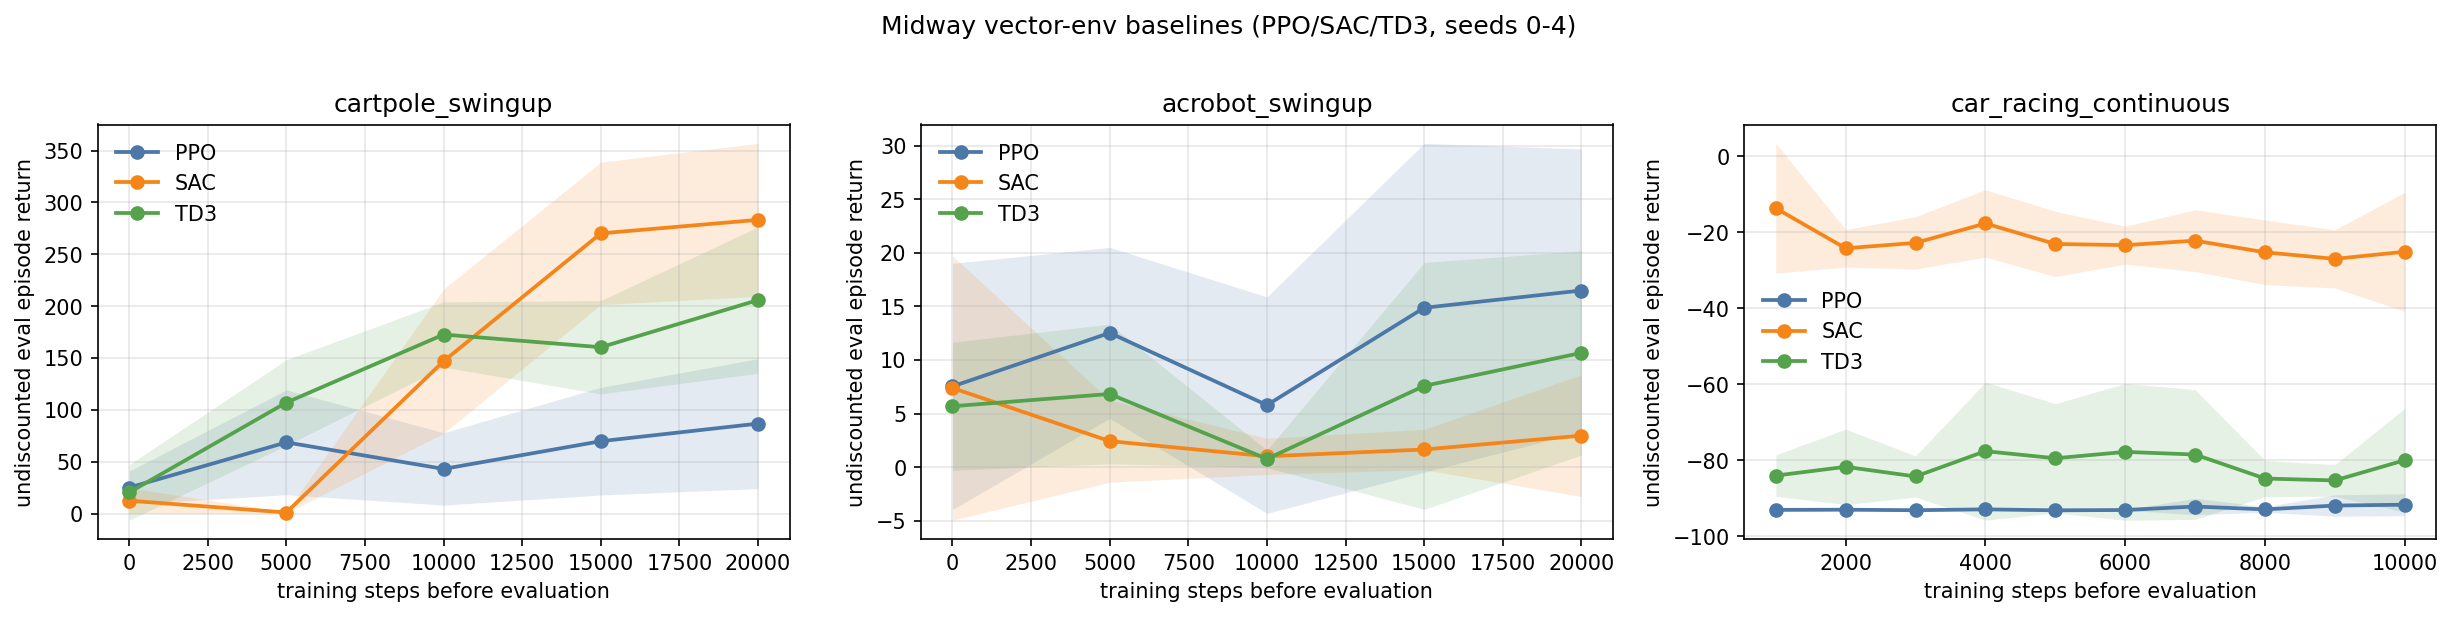
\includegraphics[width=\linewidth]{../figures/midway/midway_vector_env_baselines.png}
  \caption{Midway PPO, SAC, and TD3 baseline learning curves for the vector-control environments.}
  \label{fig:midway-vector-baselines}
\end{figure}


\subsection{Stability and Variation}
\label{sec:stability-variation}

The results also show variation across seeds and evaluation points. This is expected in reinforcement learning, where initialization, exploration, and environment interaction can affect the learning trajectory.

The stability summaries should not be used to identify a generally most stable algorithm across all tasks. They describe the variation observed in the specific midway runs. An algorithm may have low variation but also low performance, while another algorithm may obtain higher final return with greater variation.

For example, SAC obtains the best final return on CarRacing at the midway budget, but it is not necessarily the least variable method. On CartPole, SAC and TD3 obtain stronger final performance than PPO, but with more variation. This supports the overall interpretation: the results are useful for validating the pipeline and identifying preliminary patterns, but they are not sufficient for final claims about robustness or generalization.

\subsection{Limitations}
\label{sec:experiment-limitations}

The midway experiments have four main limitations. First, the training budgets are short. The results therefore show early learning behaviour rather than necessarily converged policies. This is particularly relevant for CarRacing, where image observations and CNN-based policy learning typically require longer training.

Second, no hyperparameter optimization was performed. Differences between PPO, SAC, and TD3 may therefore reflect both algorithmic differences and the selected baseline configurations.

Third, the GRPO-control method has not yet been implemented in these experiments. This section therefore does not evaluate the final proposed method. Instead, it establishes the baseline foundation against which the final method should be compared.

Fourth, the project uses two implementation paths: ObjectRL for vector-control environments and project-side CNN agents for CarRacing. This is a practical choice at the midway stage, but it also means that differences between vector-control and CarRacing reflect not only environment difficulty, but also differences in observation type and model architecture.

\subsection{Transition to the Final GRPO Stage}
\label{sec:transition-final-grpo}

The main conclusion from the experiments is that the baseline foundation is now in place. All PPO, SAC, and TD3 runs have been completed on all three environments with five seeds, and the results are collected in a validated result pipeline.

In the final project stage, the same experimental structure should be reused for GRPO-control. GRPO should be evaluated on the same environments, with the same seed structure and the same evaluation metric. This will make the final comparison between GRPO, PPO, SAC, and TD3 more consistent and reproducible.

The midway experiments therefore do not answer the full research question of the project. Instead, they establish the infrastructure, baseline performance, and result validation on which the final GRPO analysis depends.
